\documentclass[usejistfm]{ieej}
\usepackage{url}
\usepackage{amsmath}
\usepackage[dvipdfmx]{graphicx}
\usepackage[dvipdfmx]{color}
\usepackage[varg]{txfonts}
\usepackage{bm}
\usepackage[caption=false]{subfig}

%\usepackage[top=0.5in]{geometry}
%\usepackage{fullpage}
%\usepackage{auto-pst-pdf}
%\usepackage{epstopdf}
%\usepackage{float}
\usepackage{subfloat}
%\usepackage{caption}
%\usepackage{axodraw4j}
%\usepackage{pstricks}


\jtitle{半導体歪ゲージを用いたハイダイナミックレンジ1軸力覚センサの開発}
%\etitle{Development of a compact high dynamic range 6-axis force/torque sensor}
\authorlist{
 \authorentry{19MM227\ \ \ 田村 龍也}{Ryuya Tamura}{s}{TRL}
 }
%\affiliate[] {埼玉大学工学部電気電子システム工学科\\
 %〒338--8570\ 埼玉県さいたま市下大久保255}
  %{Saitama\ University \\
  %255, Shimo-ohkubo, Sakura-ku\ Saitama\ 338--8570}
\begin{document}
\begin{abstract}

%This paper proposes a compact High Dynamic Range(HDR) 6-axis Force/Torque(F/T) sensor.
It is important for robots to acquire environmental information with an HDR F/T sensor to perform various operations.
However, it is a problem that the F/T sensor with HDR is too large to attach to a robot.
Therefore, the compact HDR 6-axis F/T sensor with a new cross-structure arch type was developed.
The F/T sensor showed linearity with respect to the general force component and it was possible to remove the multiaxial interference component by calibration.
It was also shown that this F/T sensor  detect 0.2N to 500N force.


%本論文では小型なハイダイナミックレンジ6軸力覚センサを提案する. 
%ロボットが様々な動作を行う上でハイダイナミックレンジな力覚センサで
%環境情報を取得することが重要である. 
%しかしながらハイダイナミックレンジを有した力覚センサはロボットに取り付ける上で
%サイズが大きいといったことが課題となっている. 
%よってクロスアーチ型を模した新しい構造の小型HDR6軸力覚センサを開発する.
%本力覚センサはおおむねの力成分に対して線形性を示し, 
%キャリブレーションを行なうことで他軸干渉成分の除去を行なえた. 
%また本力覚センサはSN比より0.2Nから500Nまでの力覚検知が可能であることが示せた.   


\end{abstract}
%\begin{jkeyword}
 %力覚センサ,ダイナミックレンジ, 小型化, 分解能
%\end{jkeyword}
%\begin{ekeyword}
 %Force/Torque sensor, Dynamic range, Miniaturization, Resolution
%\end{ekeyword}
\maketitle


\section{まえがき} 

ロボットの活躍領域は近年急速に拡大しており, 
それとともに普及率も指数関数的に上昇している. 
この背景は, 従来は自動車や家電など製造を行う産業用途での活躍が主であったが, 
現在は医療, 介護やサービス業などの第三次産業に有効性が見込まれ, 
協働ロボット等が多く開発されていることからもわかる.

協働ロボットの中でも特に人間を支援または人間の代替として活動するロボットが注目されている. 
これらのロボットには環境適応力が求められ, 環境情報の取得が必要不可欠となっている.
中でも力覚情報は多様な動作の実現のためには必須だと考えられ, 
実際DENSOの多関節ロボット\cite{denso}の安定した作業やASIMO\cite{asimo}のお茶を注ぐ動作, 
ROBEAR\cite{ROBEAR}の人を持ち上げるといった動作も力覚センサを用い, 
力覚情報を取得することで実現している.

これまでの力覚センサは, 発生する力の大きさに合わせて, 測定に際し
適切なレンジの力覚センサを選出し使用されてきた. 
しかし多種多様な動作を一台のロボットで実現させる場合, それに導入する力覚センサは
レンジが限定的なものではなく, よりハイダイナミックレンジ(HDR:High Dynamic Range)で
あることが求められる. 
また, HDRなだけではなく, ロボットに取り付け可能なサイズであることが求められる. 

このような需要に対し, Jiangらは低剛性起歪体と高剛性起歪体を組み合わせた1軸\cite{Jiang2015}, 2軸\cite{jiang2013}
の力情報を検知可能なHDR力覚センサを提案した. 
また起歪体を用いず, 水晶振動子による圧電効果を利用しHDRで力覚検知を可能にした
1軸のセンサも提案されている\cite{murozaki2014miniaturized}.

さらに1軸, 2軸での検知のみであったHDR力覚センサに対し, Okumuraらは6軸の力情報を取得可能な
HDR力覚センサ(size:150×150×45 mm)を提案した\cite{okumura2018high}. 
これはそれぞれが6軸の力情報を取得できる低剛性起歪体と高剛性起歪体を二段に重ね合わせた構造をしており, 
0.01Nから1000Nまでの力覚検知が可能である. 従来の10倍以上のダイナミックレンジを
有した力覚センサとなった. 

%力覚センサは外力によって生じる構造体(以下, 起歪体)の変形量をセンシング素子により検知し,
%その変形量を元に外力の推定を行なう. 
%センシング素子により力覚センサの測定方式は異なり, 
%ひずみゲージ式\cite{yoshikawa1989six}%\cite{nishiwaki2002six}\cite{Liang2010}, 
%静電容量式\cite{Beyeler2009}, 
%光学式\cite{Kim2013a}%\cite{su20093}\cite{polygerinos2010novel}
%など様々な検出方法が実用化されている. 

%基本的に力覚センサの測定レンジは起歪体の剛性により決まり, 
%低剛性の起歪体は小さな力の検出が, 高剛性の起歪体は大きな力の検出が可能である. 
%しかしこれは反対に, 1つの起歪体だけでは小さな力と大きな力の検出を行なえないことを示唆している. 
%起歪体の変形を検知するという原理上, 分解能と定格荷重はトレードオフの関係にあり, 従来の力覚センサの
%ダイナミックレンジ(測定可能な力の最小値と最大値の比)には制限が生じる. 

しかし, 提案されてきたHDR力覚センサはセンサ自体のサイズが大きく, 
先述したようなロボットに導入する上で大きな問題となる.

これに対し我々は起歪体の構造自体を工夫することでHDRと小型化の両立を図るセンサの提案をした. 
このセンサは低剛性起歪体の形状がクロスアーチ型となっており, 
高剛性起歪体の隙間にフィットする構造となっている. センササイズは〇と小型化に成功し, 
測定レンジは〇を確保出来た.
しかし, 低荷重域での測定が不向きであることや, 
従来センサのHDRの広さを保つことが出来なかった. 

%この問題に対し, Okumuraらはさらに, 低剛性起歪体と高剛性起歪体を一層に集約した
%樹脂製のHDR6軸力覚センサ(size:100×100×30 mm)を
%提案した\cite{Okumura}. 樹脂製HDR6軸力覚センサは起歪体を水平に配置することで 
%センサの高さが低くなる. また高剛性起歪体の梁を短く設計したことで体積が小さくなった. 
%しかし, 樹脂製HDR6軸力覚センサは素材の特性上, クリープ現象や応力緩和といった金属製センサではあまり見られなかった
%特性が生じた. 

このことから, 小型かつHDRを有した力覚センサの実現には, 
被測定材料にあたるセンサ構造自体を工夫するのではなく, 
センシング部分の改革が必要であると考えた. 

そこで本論文では, HDRを実現する新たなる手法として, 半導体歪ゲージと金属箔歪ゲージを併用した
小型で単純な構造の力覚センサを提案する. 
従来は剛性の異なる起歪体を多段に使用することで実現していたHDRを, 
本センサでは単純な起歪体構造(片持ち梁)上に感度の異なるひずみゲージを導入すること(のみ)でHDRを実現した. 

%以下に本論文の構成を示す. まず,2章で力覚センサに関連する原理を述べる.
%次に3章では提案する小型HDR6軸力覚センサを示し,4章でシミュレーションによって, 提案する力覚センサの
%挙動と設計の妥当性を確認する. 5章では実際に製作した力覚センサの有用性を確認するため行なった性能試験の結果を述べ, 
%最後の6章でまとめとする. 

\section{力覚センサの原理}
力覚センサは力覚情報を測定するセンサである. 
力覚情報を測定するためには, 被測定材料のひずみ, 変化量, または素子の特性変化等を電気信号に
変換する必要があり. 
本研究で提案する力覚センサはひずみゲージ式の力覚センサである. 

\subsection{ひずみゲージ}
材料に引張力(または圧縮力)$P$が加わる時, これに対応する応力$σ$が材料内部に発生する.
ここでこの応力に比例した引張ひずみ(または圧縮ひずみ)が発生し, 長さ$L$の材料は
$L + \Delta L$(または$L - \Delta L$)に変形する. 
この時の$L$と$\Delta L$の割合をひずみと呼ぶ. 

ひずみゲージはこのひずみを電気信号として検出することのできるセンシング素子のことである. 

本研究で使用するひずみゲージは金属箔ひずみゲージと半導体ひずみゲージの二種類である. 
ひずみの値はとても小さな値で変化するものであり, 
金属箔ひずみゲージの場合は

\subsection*{金属箔ひずみゲージ}
\subsection*{半導体ひずみゲージ}

\subsection{起歪体}

%6軸力覚センサとはデカルト座標系における$x, y, z$軸方向の力($Fx, Fy, Fz$)と力のモーメント($Mx, My, Mz$)の大きさを
%測定するセンサである. 本研究では一般的に広く利用されているひずみゲージ式を採用した. 

%力覚センサは起歪体に生じるひずみの変化量を力情報へと変換する. 
%力覚センサに印加される荷重\textbf{\textit{L}}($F$[N], $M$[Nm])と
%ひずみ出力\textbf{\textit{S}}[$\mu$m/m]は次のように表せる. 
%\begin{eqnarray}
%  \bm{L} = {[F_x, F_y, F_z, M_x, M_y, M_z]}^{\top} \\
%  \bm{S} = {[ S_1, S_2, S_3, S_4, S_5, S_6 ]}^{\top}
%\end{eqnarray}
%荷重$\bm{L}$とひずみ出力$\bm{S}$は荷重-ひずみ行列$\bm{C}$によって次のように関係付けられる. 
%\begin{eqnarray}
%  \bm{S} = \bm{C}\bm{L}
%\end{eqnarray}
%また, 荷重-ひずみ行列$\bm{C}$の逆行列を用いると
%\begin{eqnarray}
%  \bm{L} = \bm{C}^{-1}\bm{S}
%  \label{eq:syuturyoku}
%\end{eqnarray}
%となる. よってひずみ出力$\bm{S}$を元に印加された荷重$\bm{L}$の計測が可能となる. 

%次に較正行列の求め方\cite{hanyu2010simplified}を述べる. ここで, すでに印加荷重$\bm{L}$と
%そのときのひずみ$\bm{S}$の値が既知であり, そのサンプル数は$n$であるとする.
%つまり, $\bm{L} = [\bm{L}^1, \bm{L}^2, \cdots , \bm{L}^n]$, $\bm{S} = [\bm{S}^1, \bm{S}^2, \cdots , \bm{S}^n]$
%が既に与えられているとする。ここで、$\bm{L}^k = [F^k_x, F^k_y, F^k_z, M^k_x, M^k_y, M^k_z]^{\top}$, $\bm{S}^k = [S^k_1, S^k_2, \cdots, S^k_i]^{\top} $
%とすると
%\begin{eqnarray}
%  \bm{C}^{-1} = \bm{L} \bm{S}^{-1} \label{eq:c}
%\end{eqnarray}
%によって$\bm{C}^{-1}$を求めることが可能である. 
%以下、簡単のため$\bm{L}$の$F_x$のみを考える。較正行列$\bm{C}$の逆行列$\bm{C}^{-1}$を
%\begin{eqnarray}
%\bm{C}^{-1} = \left[
%   \begin{array}{cccc}
%     a_{11} & a_{12} & \ldots & a_{16} \\
%     a_{21} & a_{22} & \ldots & a_{26} \\
%     \vdots & \vdots & \ddots & \vdots \\
%     a_{61} & a_{62} & \ldots & a_{66}
%   \end{array}
% \right]
%\end{eqnarray}
%とすると、$k$サンプル目の$F^k_x$の予測値$F^{k\ast}_x$は
%\begin{eqnarray}
%   F^{k\ast}_x = a^k_{11} S^k_1 + a^k_{12} S^k_2 + \cdots + a^k_{16} S^k_6
%\end{eqnarray}
%と表される。
%式\eqref{eq:c}は実際の印加荷重と予測値の残差二乗和
%\begin{eqnarray}
%  \sum_{k=0}^{n} d^2_k = \sum_{k=0}^{n} {\left(F^k_x - F^{k\ast}_x \right)}^2
%\end{eqnarray}
%が最小となるような定数$[a_{11}, a_{12}, \ldots, a_{16}]$を最小二乗法で導出するのと等価である. 
%ことで、$\bm{C}^{-1}$の$F_x$に寄与する部分を求めることができる。他の軸も同様に求めることができ、合わせることで較正行列$\bm{C}$の逆行列$\bm{C}^{-1}$を求めることができる。


\section{HDR1軸力覚センサの設計}
\subsection{起歪体の構造}
提案する力覚センサの構造とひずみゲージ貼り付け位置をFig.~\ref{fig:sensor}に, 
起歪体の寸法をTable~\ref{tb:size}に示す.
本研究ではセンシング部分の提案によるHDRの原理的検証を目的としているため, 
起歪体の構造は非常に単純な片持ち梁を採用した. 
また, 大荷重に耐えられるよう起歪体の材料は剛性の高い超々ジュラルミンを採用した. 

%\begin{figure}[b]
%  \begin{center}
%    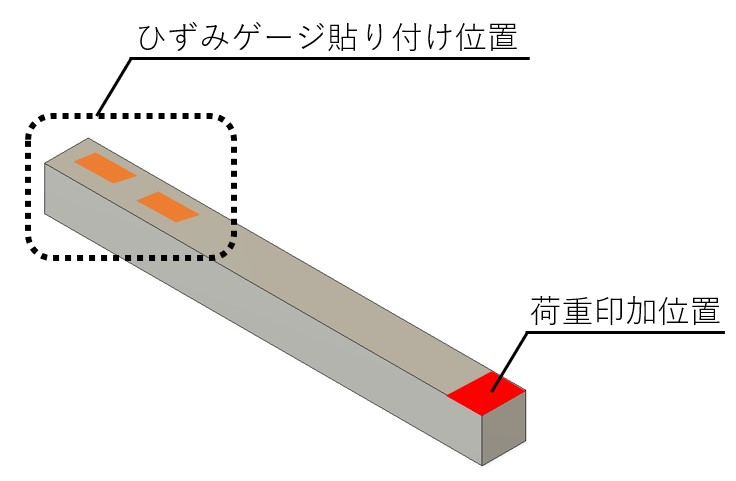
\includegraphics[width=6.0cm]{pic/hari.jpg}
%    \caption{HDR1軸力覚センサのCADモデル}\label{fig:sensor}
%  \end{center}
%\end{figure}

\begin{table}[h]
  \caption{起歪体の寸法 [mm]}\label{tb:size}
  \begin{center}
   \begin{tabular}{ c c c c }
    \hline
     & Length & Width & Height  \\
    \hline
    Cantilever beam & 100 & 10 & 10  \\
    \hline   
   \end{tabular}
  \end{center}
 \end{table}

\subsection{ひずみゲージ貼り付け位置}
有限要素法シミュレーションによる起歪体のひずみ分布をFig.~\ref{fig:sim}に示す.

ひずみゲージは被測定対象のひずみが伝達することにより抵抗変化が生じる
センシング素子である. 
ひずみの変化は大変微小であるため, ひずみゲージの貼り付け位置は
測定対象のよりひずみやすい部分に貼り付けることが求められる. 
よって有限要素法シミュレーションにより任意の荷重を印加, 
この時のひずみ分布をもとに貼り付け位置を決定した. 

また, このシミュレーション結果より得られた本センサの定格荷重と
定格荷重印加時の安全率のパラメータをTable~\ref{tb:kajuu}に示す.

\begin{table}[h]
  \caption{定格荷重と安全率}\label{tb:kajuu}
  \begin{center}
   \begin{tabular}{ c c }
    \hline
    定格荷重 $F$[N] & 安全率 \\
    \hline
    200.0 & 1.145 \\
    \hline   
   \end{tabular}
  \end{center}
 \end{table}

\begin{figure}[b]
  \centering
  \begin{tabular}{c}
    \begin{minipage}{0.5\hsize}
      \begin{center}
        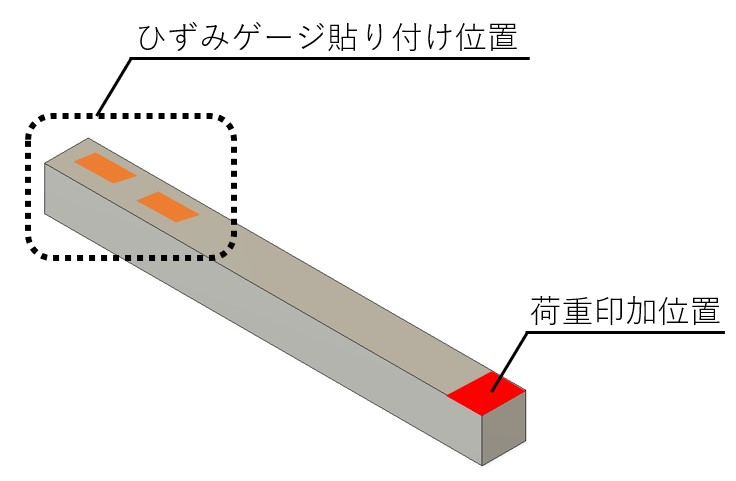
\includegraphics[scale=0.2]{pic/hari.jpg}
        \hspace{1.cm} 
        \footnotesize{起歪体}
      \end{center}
    \end{minipage}
        \begin{minipage}{0.51\hsize}
      \begin{center}
        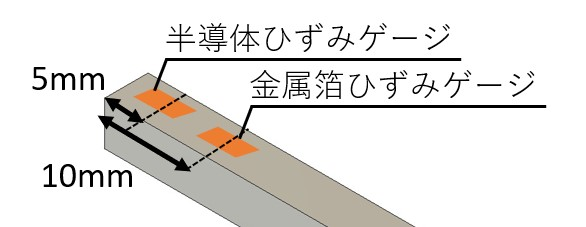
\includegraphics[scale=0.29]{pic/hizumi.jpg}
        \hspace{1.6cm} 
        \footnotesize{ひずみゲージの貼付位置}
      \end{center}
    \end{minipage}
  \end{tabular}
  \caption[]{HDR1軸力覚センサ}\label{sensor}
\end{figure}

\begin{figure}[h]
  \begin{center}
    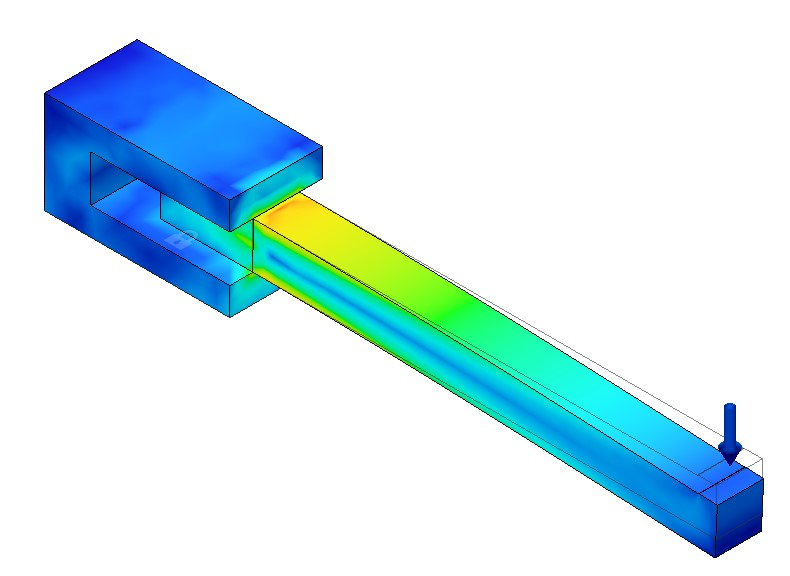
\includegraphics[width=5.5cm]{pic/simHizumi.jpg}
    \caption{有限要素法シミュレーションによる結果}\label{fig:sim}
  \end{center}
\end{figure}

\subsection{測定回路系の構成と計測レンジ}
ひずみを取得するための測定回路を%Fig.~\ref{fig:kairo}
に示す. 
ひずみの変化を受けて抵抗値が変位するひずみゲージは, 
ホイートストンブリッジ回路に接続される. 
ブリッジ電圧を読み取り, A/D変換された値がカットオフ周波数$fc = 10$HzのLPFを通って
USB接続されたPCに出力されることで, ひずみの計測が行える. 

ここで, 金属箔ひずみゲージと半導体ひずみゲージの適用レンジ, 
分解能を%Fig.~\ref{fig:kairo}
に示す. 
今回使用したひずみアンプはPCD-400Aで, このひずみアンプの測定レンジは
最大$20000×10^{-6}$である. Table~\ref{tb:gage}に記したように
金属箔, 半導体ひずみゲージのひずみ限界はそれぞれ$20000, 3000×10^{-6}$であるが, 
出力として得られる値は, 起歪体に生じたひずみのゲージ率倍されたものである. 
よって, 金属箔ひずみゲージでは$10000×10^{-6}$までのひずみを出力として得ることができ, 
半導体ひずみゲージでは金属箔ひずみげーじでノイズに埋もれてしまう
低荷重域の値を$110×10^{-6}$まで出力値として得ることができる. 
このひずみのレンジを印加荷重のレンジに置き換えると%Fig.~\ref{fig:kairo}
に示したレンジとなり, ゲージ率の異なるひずみゲージを併用することでHDRを
有した力覚センサを設計することが可能であると見込める. 





\section{性能試験}
実際に製作した力覚センサに対する性能試験の結果について述べる. 
今回の試験は各起歪体ごとに行なった. 
ストッパ機構の働きを確認する試験は$F_z$成分の結果を示す. 

製作した力覚センサをFig.~\ref{fig:jissai}に示す.

\begin{figure}[h]
  \centering
  \subfloat[低剛性起歪体]{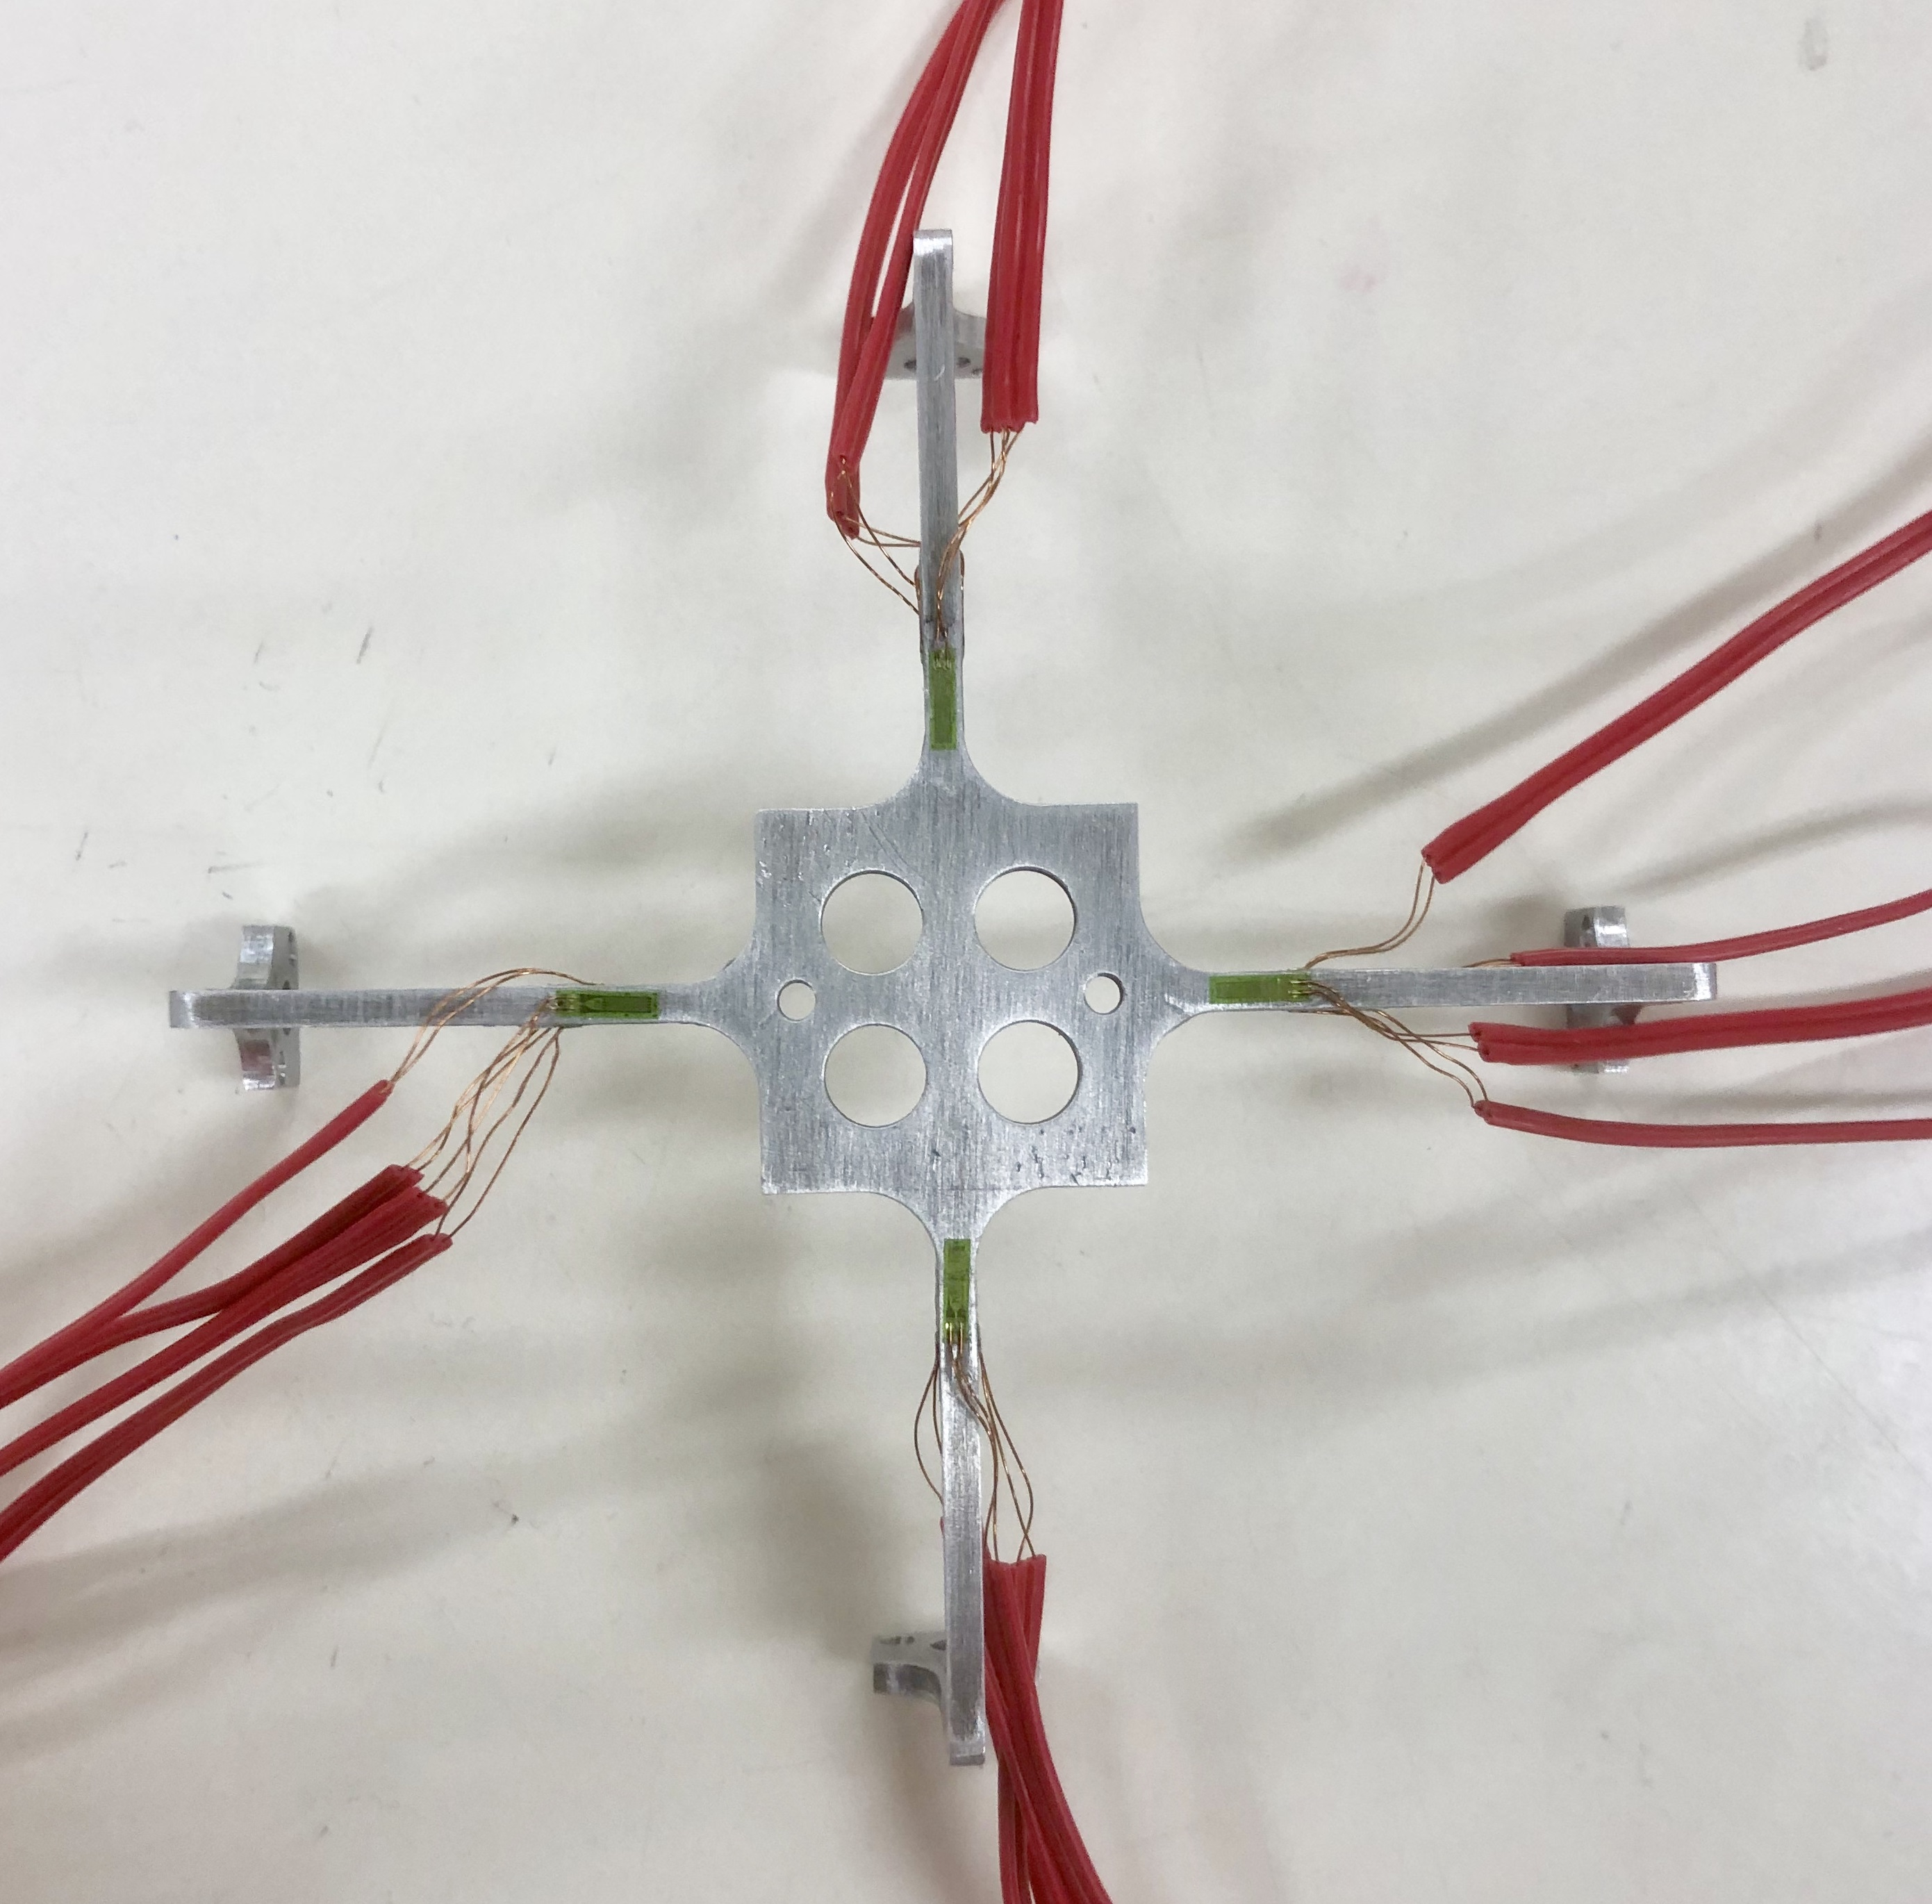
\includegraphics[width=4.2cm]{pic/real_L.jpg}}
  \subfloat[高剛性起歪体]{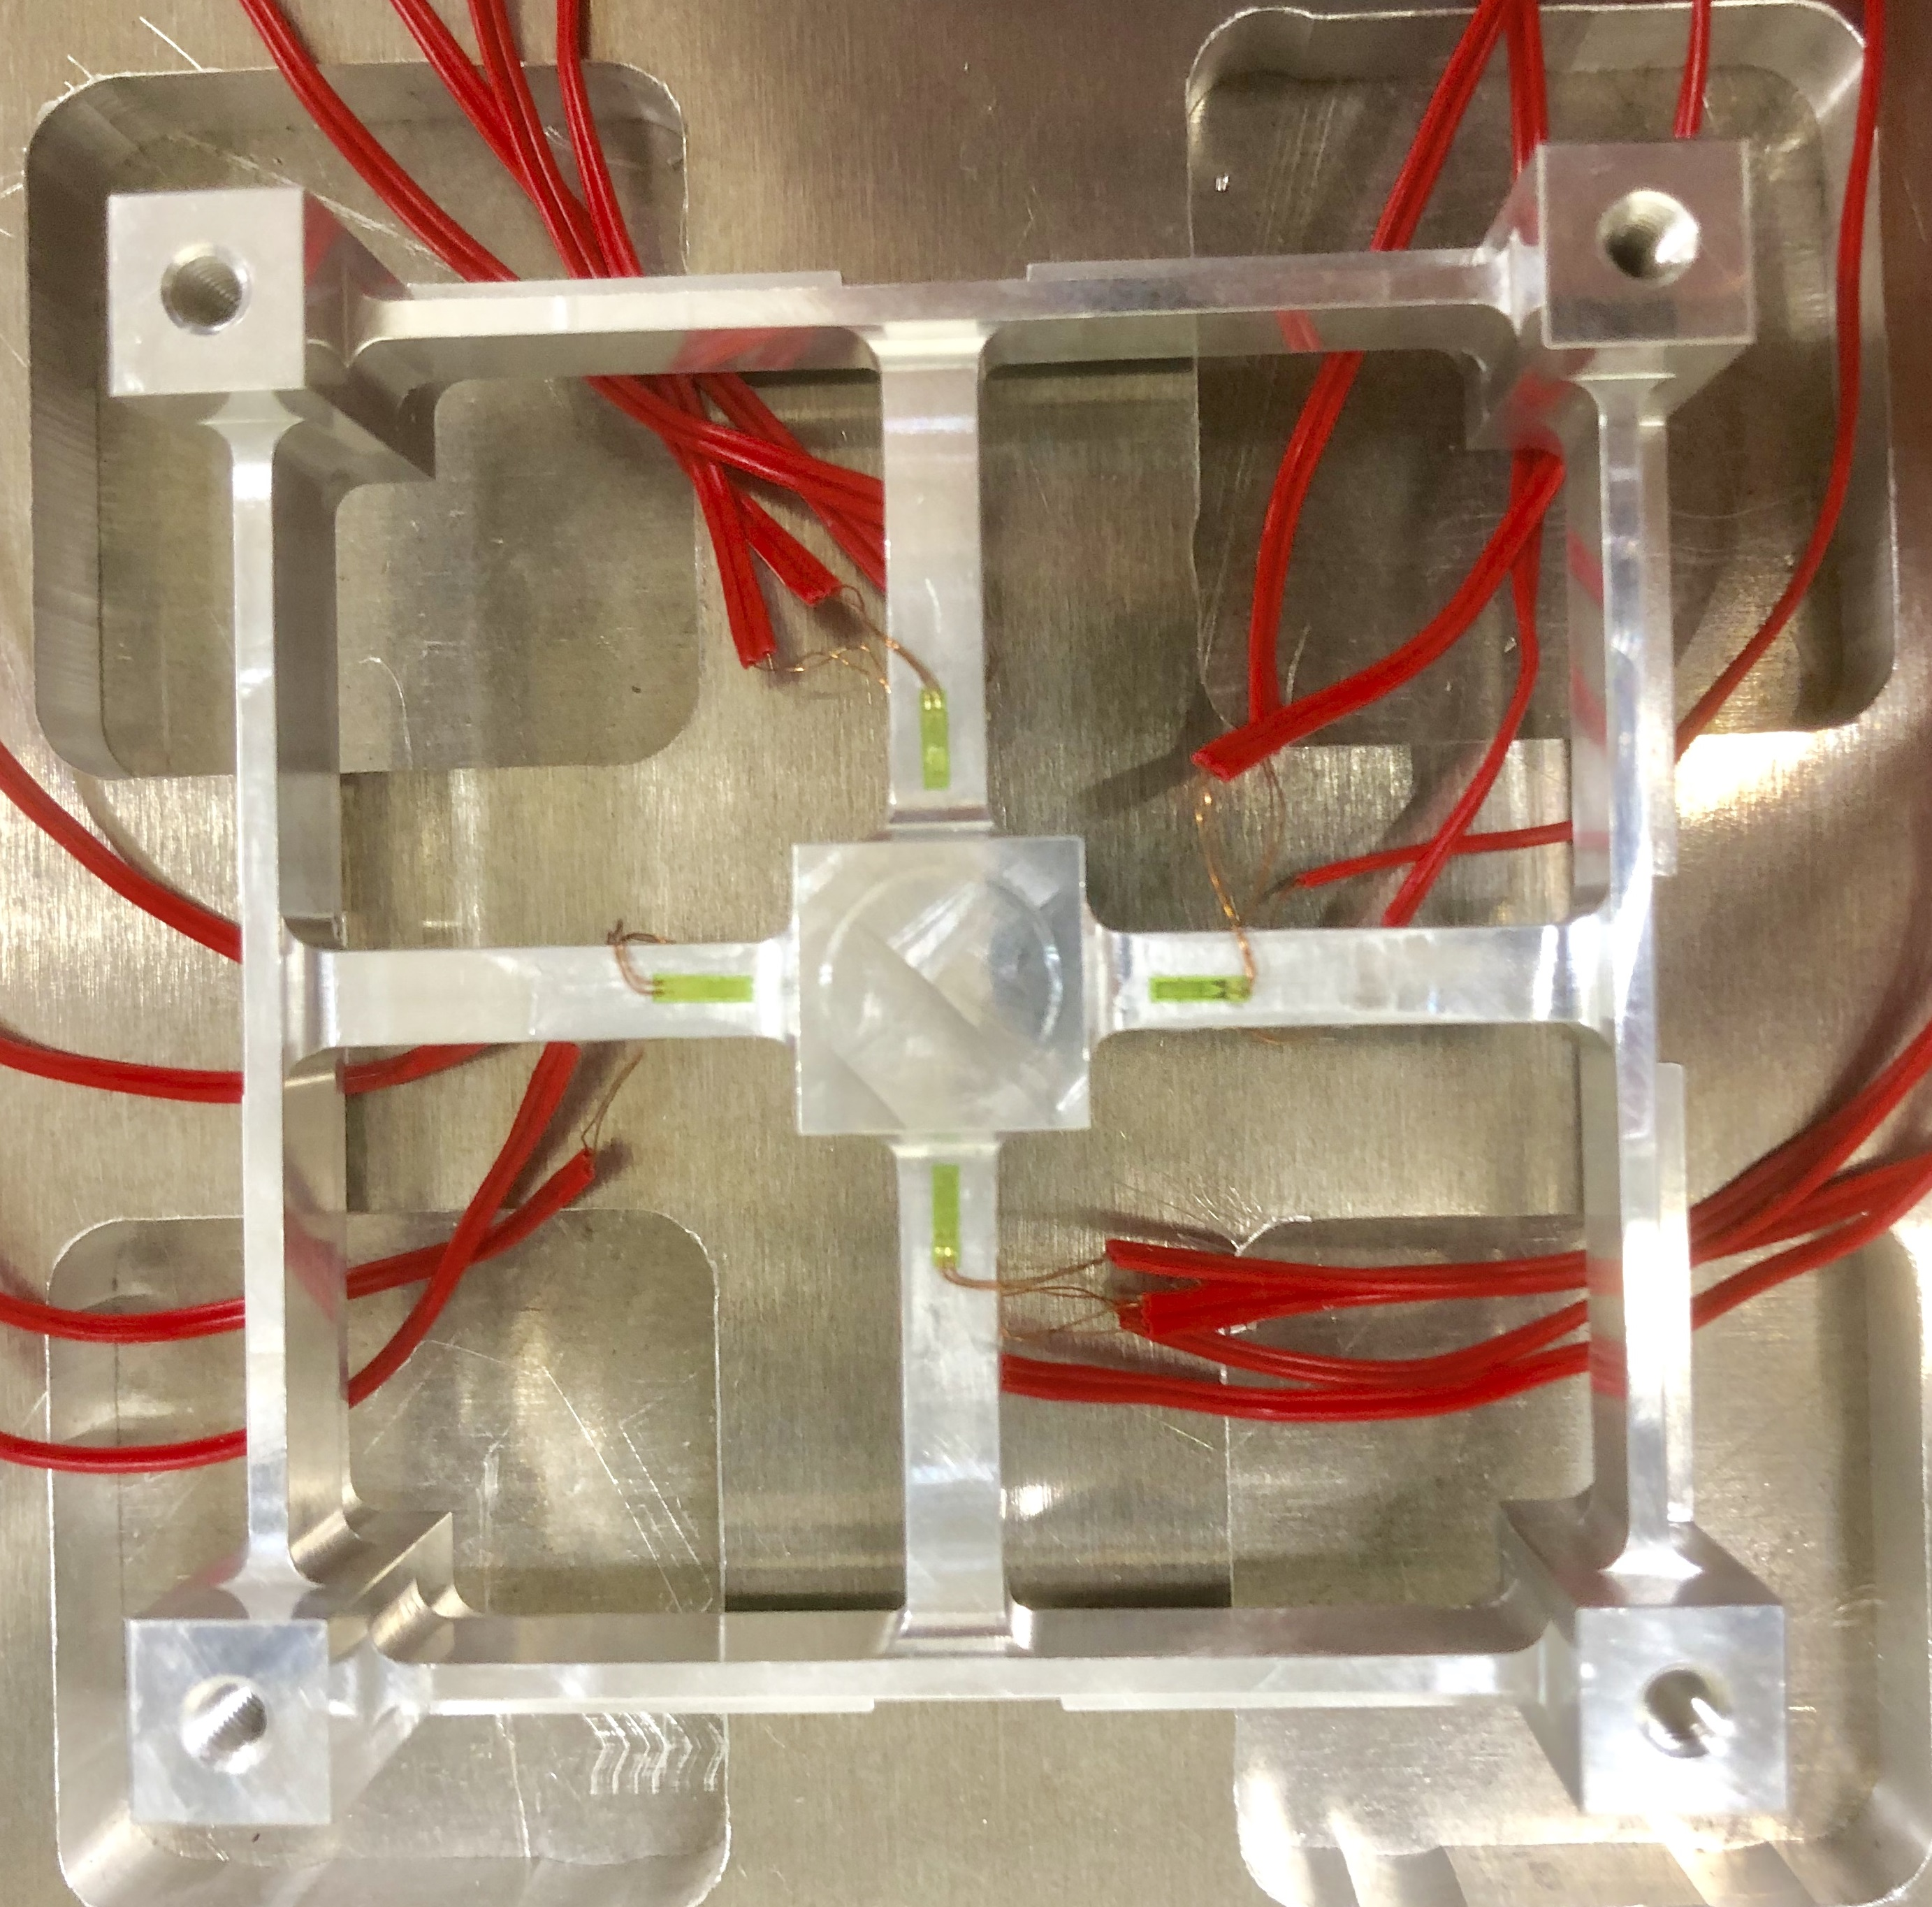
\includegraphics[width=4.2cm]{pic/real_H.jpg}}\\
  \caption[]{製作した小型HDR6軸力覚センサ}\label{fig:jissai}
\end{figure}

\subsection{非線形性・他軸干渉試験}
力覚センサは荷重-ひずみ変換行列を用いて印加荷重を算出する. 
印加された荷重に対する出力値の非線形性や, 
印加された荷重以外の成分の出力が応答する他軸干渉は
力覚センサの性能に関わる重要な指標である. 
 
\subsubsection*{低剛性起歪体}
任意に印加した荷重とひずみ出力の関係から式~\eqref{eq:c}をもとに
正負それぞれの荷重-ひずみ変換行列を算出した. 
\begin{eqnarray}
  \bm{C}^{-1}_{+low} = \left[
 \scalebox{0.7}{$\displaystyle
  \begin{array}{cccccc}
 13.4  &-9.8   &3.3  &-2.71  &-0.2 &14.2   \\
 7.7   &32.3   &-2.5 &5.1    &-6.4 &-9.5   \\
 0     &-2.9   &8.1  &0.1    &1.1  &1.5    \\
 0     &-0.1   &0    &0.1    &0    &0      \\
 0.1   &0      &0    &0      &0.1  &0.1    \\
 -0.1  &-0.1   &0    &0      &-0   &0.2  
 \end{array}$} 
 \right]
 \times 10^{-3} 
 \end{eqnarray}
 
 \begin{eqnarray}
   \bm{C}^{-1}_{-low} = \left[
     \scalebox{0.7}{$\displaystyle
  \begin{array}{cccccc}
   40.1  &12.6 &10.4 &-0.1 &-10.5  &17.7    \\
   -13.7 &16.3 &-4.2 &3.8  &-0.1   &-15.2   \\
   6.3   &1.7  &9    &0.6  &-1.3   &3.1     \\
   0     &-0.1 &0    &0.1  &0      &0       \\
   0.2   &0.1  &0.1  &0    &0      &0.1     \\
   0.2   &0.2  &0.1  &0    &-0.1   &0.2  
 \end{array}$}
 \right]
 \times 10^{-3} 
 \end{eqnarray}

算出した荷重-ひずみ変換行列により変換した低剛性起歪体の荷重出力を
Fig.~\ref{fig:kajyuLow}に示す.
6軸ともに線形的な出力結果が得られた. 
しかし, $F_x, F_z, M_z$の結果を見ると, 他軸干渉成分が較正しきれていないことが
確認できる. 

\subsubsection*{高剛性起歪体}
低剛性起歪体同様に, 任意に印加した荷重とひずみ出力の関係から式~\eqref{eq:c}をもとに
正負それぞれの荷重-ひずみ変換行列を算出した. 

\begin{eqnarray}
  \bm{C}^{-1}_{+high} = \left[
    \scalebox{0.7}{$\displaystyle
 \begin{array}{cccccc}
10.3  &-0.2   &5.3  &-3.9  &0.4  &3.7   \\
-0.2  &6.6    &0.5  &0     &-0.4 &-0.1  \\
-0.7  &-0.6   &7.1  &0.3   &0.8  &-0.2  \\
0     &-0.2   &-0.1 &0.2   &0    &-0.1  \\
0.3   &0      &0.2  &-0.1  &0.2  &0.1   \\
0     &0      &0    &0     &0    &0.3  
\end{array}$}
\right]
\times 10^{-3}
\end{eqnarray}

\begin{eqnarray}
  \bm{C}^{-1}_{-high} = \left[
    \scalebox{0.7}{$\displaystyle
 \begin{array}{cccccc}
  10.1  &-0.7 &3.9  &-3.8 &0    &3.7   \\
  0     &6.9  &0.6  &-0.1 &-0.4 &0     \\
  -0.1  &-0.1 &6.9  &0.1  &0.8  &0     \\
  0     &-0.2 &-0.1 &0.2  &0    &-0.1  \\
  0.3   &0    &0.1  &-0.1 &0.1  &0.1   \\
  0     &0    &0    &0    &0    &0.3  
\end{array}$}
\right]
\times 10^{-3}
\end{eqnarray}

算出した荷重-ひずみ変換行列により変換した高剛性起歪体の荷重出力を
Fig.~\ref{fig:kajyuHigh}に示す. 
$F_z, M_y$以外は比較的良好な線形性を有している. 
他軸干渉成分に関しては, モーメント成分の結果に比べ力成分の他軸干渉が大きく見られる.

さらに各成分に対する非線形性・他軸干渉に関して数値的評価を行う. 
非線形性・他軸干渉はそれぞれ以下の式によって導出した. 
結果をTable.~\ref{tb:hisennkeisei}, Table.~\ref{tb:tajikukannsyou}に示す. 

\begin{eqnarray}
  NL^{F_x} = \frac{L^{F_x}_{true} - L^{F_x}_{out}}{L^{F_x}_{rated}}
\end{eqnarray}

\begin{eqnarray}
  \scalebox{0.7}{$\displaystyle
  CC^{F_x} = \sqrt{\Biggl(\frac{L^{F_y}_{out}}{L^{F_y}_{rated}}\Biggr)^2 + \Biggl(\frac{L^{F_z}_{out}}{L^{F_z}_{rated}}\Biggr)^2 + \Biggl(\frac{L^{M_x}_{out}}{L^{M_x}_{rated}}\Biggr)^2 + \Biggl(\frac{L^{M_y}_{out}}{L^{M_y}_{rated}}\Biggr)^2 + \Biggl(\frac{L^{M_z}_{out}}{L^{M_z}_{rated}}\Biggr)^2}
$}
\end{eqnarray}
ここで, $L_{true}$は印加荷重の真値, $L_{out}$はセンサ出力, $L_{rated}$は定格荷重, 上添え字は6成分を表す. 

低剛性起歪体は$M_y$以外の軸では算出結果からも線形性が示された. 
高剛性起歪体は低剛性起歪体と比較すると非線形的であるが, 
Fig.~\ref{fig:kajyuHigh}で確認できた結果同様に$F_z, M_y$以外の軸は
線形性が示された. また他軸干渉においては低剛性起歪体の結果が
大きい数値を示している. これは主軸自体の出力値が小さい分, 
他軸成分が大きく干渉してしまっていると考えられる. 
\begin{table}[h]
  \caption{非線形性[\%R.O.]\label{tb:hisennkeisei}}
  \begin{center}
   \begin{tabular}{ c c c c c c c }
    \hline
     & $F_x$ & $F_y$ & $F_z$ & $M_x$ & $M_y$ & $M_z$  \\
    \hline
    Low & 1.05 & 2.09 & 0.15 & 21.3 & 5.90 & 0.54 \\
     \hline
    High & 2.86 & 2.64 & 7.84 & 1.95 & 5.84 & 2.88  \\
    \hline   
   \end{tabular}
  \end{center}
 \end{table}

 \begin{table}[h]
  \caption{他軸干渉[\%R.O.]\label{tb:tajikukannsyou}}
  \begin{center}
   \begin{tabular}{ c c c c c c c }
    \hline
     & $F_x$ & $F_y$ & $F_z$ & $M_x$ & $M_y$ & $M_z$  \\
    \hline
    Low & 10.5 & 7.23 & 20.1 & 21.3 & 13.3 & 19.9  \\
     \hline
    High & 3.57 & 21.1 & 23.9 & 1.2 & 3.22 & 0.99 \\
    \hline   
   \end{tabular}
  \end{center}
 \end{table}

\subsection{SN比と測定レンジ}
Fig.~\ref{fig:sn}に$F_z$成分のSN比の推移を示す. 
この結果は高周波ノイズ(0.3\%R.O.), 非線形性, 他軸干渉を考慮したものとなっている. 
高剛性起歪体のみの結果を見るとSN比は低剛性起歪体の測定レンジ内で0dBを下回っている.  
低剛性起歪体と高剛性起歪体を組み合わせた場合では0.2NでのSN比が0dBを上回る結果となった. 
この結果より, 高剛性起歪体のみでは低剛性起歪体を用いることで, 1つのセンサとして測定が
可能となっていることが分かる.  
よって本力覚センサは0.2Nから500Nの測定レンジを有していることが示された. 

\subsection{過負荷防止機構の働き}
$F_z$成分の荷重を印加し過負荷防止機構の働きを確認した.
Fig.~\ref{fig:stop}に印加された荷重に対する低剛性起歪体と高剛性起歪体のひずみ出力を示す.
低剛性起歪体のひずみ出力は定格荷重として設定された50Nが印加されるまでは上昇し, 
それ以降はひずみ出力の上昇が見られない. 高剛性起歪体のひずみ出力は50N以上の荷重印加以降,
ひずみ出力が大きくなっているのが確認できる. よって過負荷防止機構が作動し, 荷重が伝達される
起歪体が切り替わっていることが確認できた. 


\section{まとめ}
小型かつHDRを有した力覚センサの開発を目的とし, 片持ち梁の起歪体に
金属箔歪ゲージと半導体歪ゲージを貼り付ける構造のセンサを提案した. 

製作したHDR1軸力覚センサの構造は非常に単純な設計で構成することが可能であり, 
半導体歪ゲージで○~○Nの範囲で分解能○の測定精度を, 
金属箔歪ゲージで○~○Nの範囲で分解能○の測定精度を示し, 
SN比より, ○Nから○Nまでの力覚検知が可能であることが示された.  
よって感度の異なる歪ゲージを併用することで, 起歪体の構造自体は単純でも
ダイナミックレンジを有した力覚センサの実現が可能であることが示された. 

今後は1軸のみで実現した本センサを6軸測定が可能なセンサへと拡張を行う. 
これにより小型かつ単純な構造のHDR6軸力覚センサの開発を目指す. 

\section*{謝辞}
この成果は, 国立研究開発法人新エネルギー・産業技術総合開発機構(NEDO)の委託業務の
結果得られたものであることをここに付記し, 関係者各位に謝意を表する. 
さらに, 本研究を進めるにあたり, 丁寧かつ熱心なご指導を賜りました辻俊明准教授, 境野翔助教をはじめ
大河原寛研究員に深謝いたします. また, 様々なご指摘をくださいました辻研究室の先輩方
および同期の皆様に感謝いたします. 


\begin{thebibliography}{10}
%\bibliographystyle{plain}    %参考文献出力スタイル(欧文)
%\bibliographystyle{junsrt}    %参考文献出力スタイル(和文)
\bibitem{denso}
力センサ有コンプライアンス機能.
\url{https://www.denso-wave.com/ja/robot/product/function/Acontact.html}
[Online; accessed 2019-02-14] 

\bibitem{asimo}
{Honda|ASIMO}.
\url{https://www.honda.co.jp/ASIMO/}.
[Online; accessed 2019-02-14] 

\bibitem{ROBEAR}
{介護支援ロボット研究用プラットフォームROBEAR}.
\url{http://rtc.nagoya.riken.jp/ROBEAR/}.
[Online; accessed 2019-02-14] 

\bibitem{yoshikawa1989six}
Tsuneo Yoshikawa and Taizou Miyazaki.
\newblock {A six-axis force sensor with three-dimensional cross-shape
  structure}.
\newblock In {\em Proc. IEEE Int. Conf. Robot. Autom.}, pp. 249--255. IEEE,
  1989.

%\bibitem{nishiwaki2002six}
%Koichi Nishiwaki, Yoshifumi Murakami, Satoshi Kagami, Yasuo Kuniyoshi, Masayuki
 % Inaba, and Hirochika Inoue.
%\newblock {A six-axis force sensor with parallel support mechanism to measure
%  the ground reaction force of humanoid robot}.
%\newblock In {\em Proc. IEEE Int. Conf. Robot. Autom.}, Vol.~3, pp. 2277--2282,
%  2002.

%\bibitem{Liang2010}
% Qiaokang Liang, Dan Zhang, Quanjun Song, Yunjian Ge, Huibin Cao, and Yu~Ge.
% \newblock {Design and fabrication of a six-dimensional wrist force / torque
%   sensor based on E-type membranes compared to cross beams}.
% \newblock {\em Measurement}, Vol.~43, pp. 1702--1719, 2010.

\bibitem{Beyeler2009}
Felix Beyeler, Simon Muntwyler, and Bradley~J. Nelson.
\newblock {A six-axis MEMS force-torque sensor with micro-Newton and
  nano-Newtonmeter resolution}.
\newblock {\em J. Microelectromechanical Syst.}, Vol.~18, No.~2, pp. 433--441,
  2009.

\bibitem{Kim2013a}
Ji~Chul Kim, Kyung~Soo Kim, and Soohyun Kim.
\newblock {Note: A compact three-axis optical force/torque sensor using
  photo-interrupters}.
\newblock {\em Rev. Sci. Instrum.}, Vol.~84, No.~12, pp. 77--80, 2013.

%\bibitem{su20093}
%Hao Su and Gregory~S Fischer.
%\newblock {A 3-axis optical force/torque sensor for prostate needle placement
%  in magnetic resonance imaging environments}.
%\newblock In {\em Proc. IEEE Int. Conf. Technol. Pract. Robot Appl.}, pp. 5--9.
%  IEEE, 2009.

%\bibitem{polygerinos2010novel}
%Panagiotis Polygerinos, Pinyo Puangmali, Tobias Schaeffter, Reza Razavi,
%  Lakmal~D Seneviratne, and Kaspar Althoefer.
%\newblock {Novel miniature MRI-compatible fiber-optic force sensor for cardiac
%  catheterization procedures}.
%\newblock In {\em Proc. IEEE Int. Conf. Robot. Autom.}, pp. 2598--2603. IEEE,
%  2010.

\bibitem{Jiang2015}
Jun Jiang, Weihai Chen, Jingmeng Liu, Wenjie Chen, and Jianbin Zhang.
\newblock {Design of a Dual-Range Force Sensor for Achieving High Sensitivity,
  Broad Bandwidth, and Large Measurement Range}.
\newblock {\em IEEE Sens. J.}, Vol.~15, No.~2, pp. 1114--1123, 2015.

\bibitem{jiang2013}
Jun Jiang, Weihai Chen, Jingmeng Liu, and Wenjie Chen.
\newblock {A cost effective multi-axis force sensor for large scale measurement
  : design , modeling , and simulation}.
\newblock pp. 188--193, 2013.

\bibitem{murozaki2014miniaturized}
Yuichi Murozaki, Kousuke Nogawa, and Fumihito Arai.
\newblock {Miniaturized load sensor using quartz crystal resonator constructed
  through microfabrication and bonding}.
\newblock {\em Robomech J.}, Vol.~1, No.~1, p.~3, 2014.

\bibitem{okumura2018high}
Daisuke Okumura, Sho Sakaino, and Toshiaki Tsuji.
\newblock {High Dynamic Range Sensing by a Multistage Six-Axis Force Sensor
  with Stopper Mechanism}.
\newblock In {\em Proc. IEEE Int. Conf. Robot. Autom.}, pp. 1--6. IEEE, 2018.

\bibitem{Okumura}
辻俊明, 奥村大輔, 境野翔.
\newblock 多段型ハイダイナミックレンジ6軸力覚センサの小型化.
\newblock  日本ロボット学会学術講演会, 2018.

\bibitem{1991}
緒方浩二郎, 柏木邦雄, 小野耕三.
\newblock 力覚センサ, 1991.

\bibitem{hanyu2010simplified}
Ryosuke Hanyu, Toshiaki Tsuji, and Shigeru Abe.
\newblock {A simplified whole-body haptic sensing system with multiple
  supporting points}.
\newblock In {\em Proc. IEEE Int. Work. Adv. Motion Control}, pp. 691--696.
  IEEE, 2010.

\bibitem{向井優2018}
向井優, 野田善之.
\newblock 六軸力覚センサの原理と構造.
\newblock 精密工学会誌, Vol.~84, No.~4, pp. 303--306, 2018.


%\bibliography{C:/Users/Kohei/Documents/library}           %data.bibから拡張子を外した名前

%\appendix
  %\input{./src/Refernces}
\end{thebibliography}

\begin{figure}[b]
  \centering
  \subfloat[$F_x$]{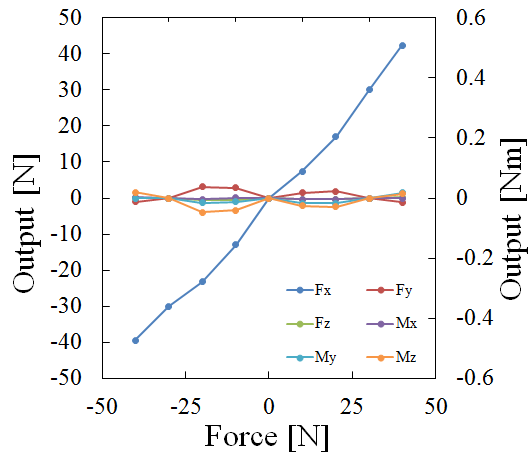
\includegraphics[scale=0.3]{pic/Fx_L.png}}
  \subfloat[$F_y$]{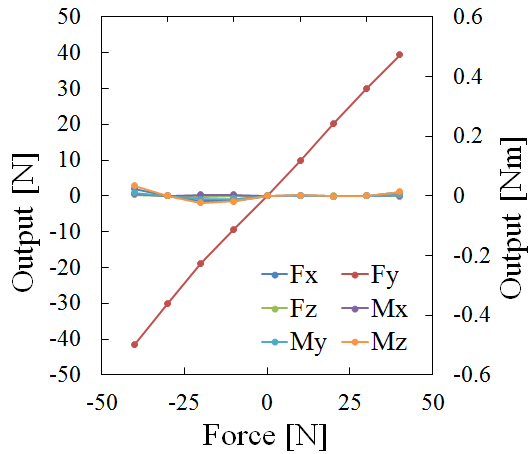
\includegraphics[scale=0.3]{pic/Fy_L.png}}\\
  \subfloat[$F_z$]{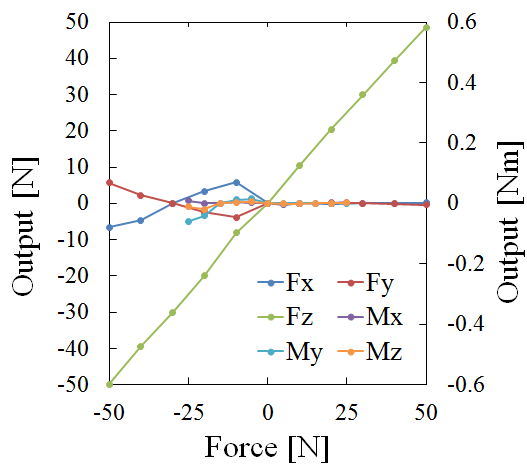
\includegraphics[scale=0.3]{pic/Fz_L.png}}
  \subfloat[$M_x$]{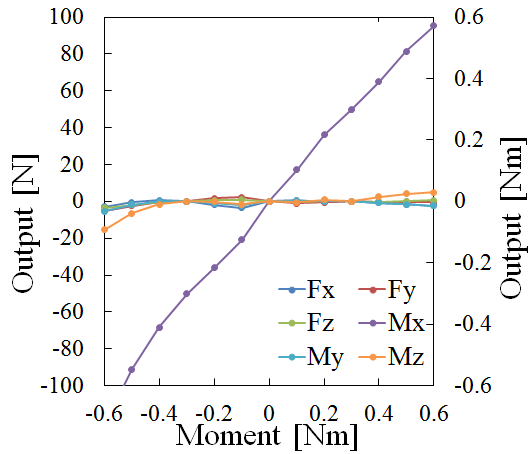
\includegraphics[scale=0.3]{pic/Mx_L.png}}\\
  \subfloat[$M_y$]{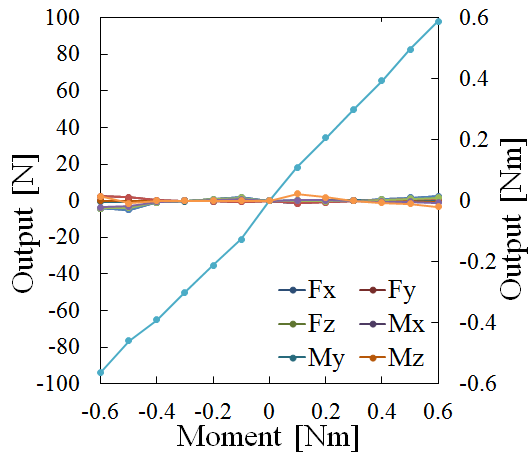
\includegraphics[scale=0.3]{pic/My_L.png}}
  \subfloat[$M_z$]{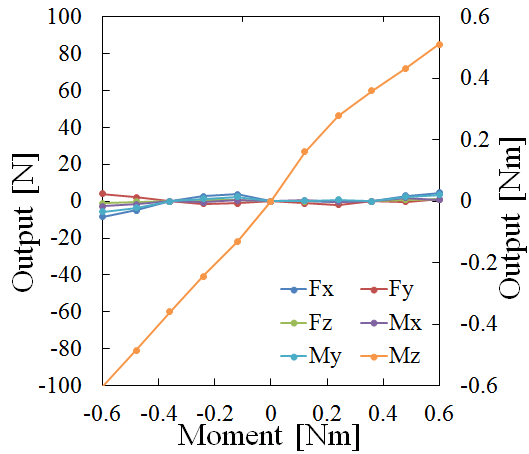
\includegraphics[scale=0.3]{pic/Mz_L.png}}\\
  \caption[]{荷重変換後の出力(低剛性起歪体)}\label{fig:kajyuLow}
\end{figure}
\begin{figure}[tb]
  \centering
  \subfloat[$F_x$]{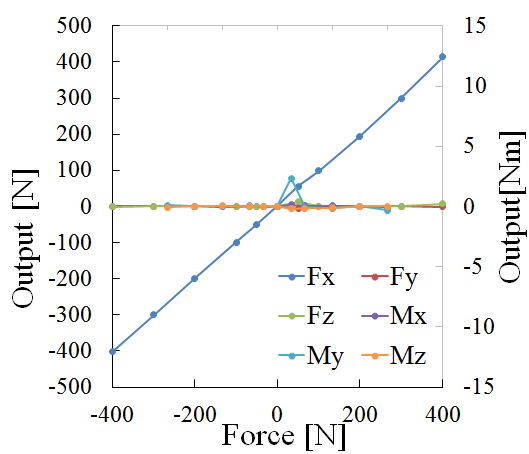
\includegraphics[scale=0.3]{pic/Fx_H.png}}
  \subfloat[$F_y$]{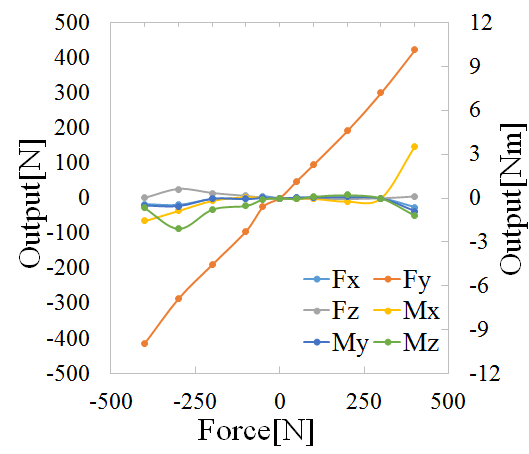
\includegraphics[scale=0.3]{pic/Fy_H.png}}\\
  \subfloat[$F_z$]{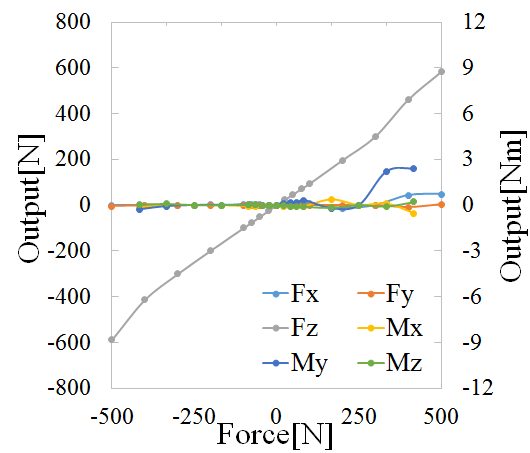
\includegraphics[scale=0.3]{pic/Fz_H.png}}
  \subfloat[$M_x$]{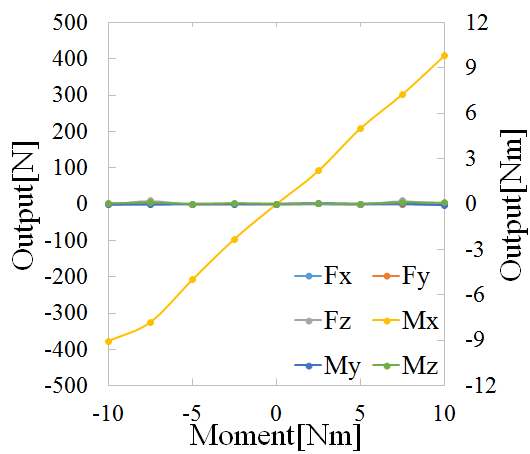
\includegraphics[scale=0.3]{pic/Mx_H.png}}\\
  \subfloat[$M_y$]{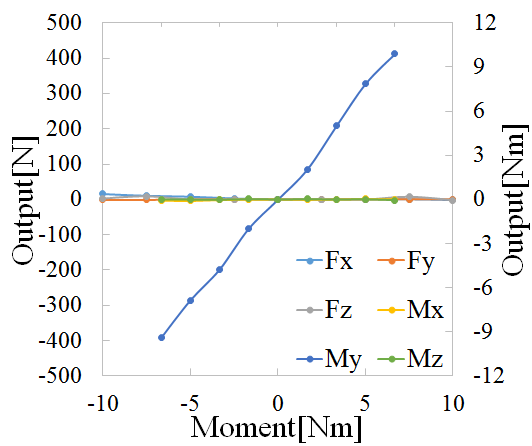
\includegraphics[scale=0.3]{pic/My_H.png}}
  \subfloat[$M_z$]{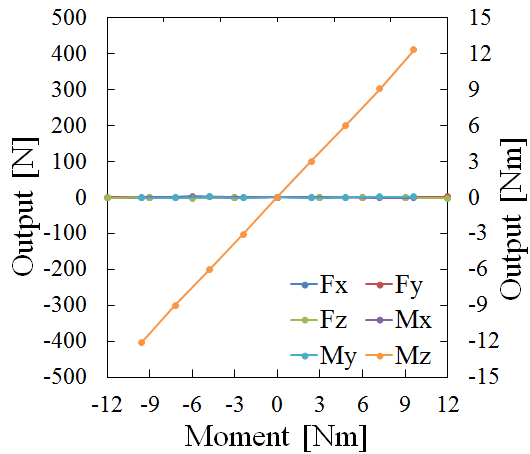
\includegraphics[scale=0.3]{pic/Mz_H.png}}\\
  \caption[]{荷重変換後の出力(高剛性起歪体)}\label{fig:kajyuHigh}
\end{figure}
\begin{figure}%[tb]
  \centering
  \subfloat[横軸:線形表示]{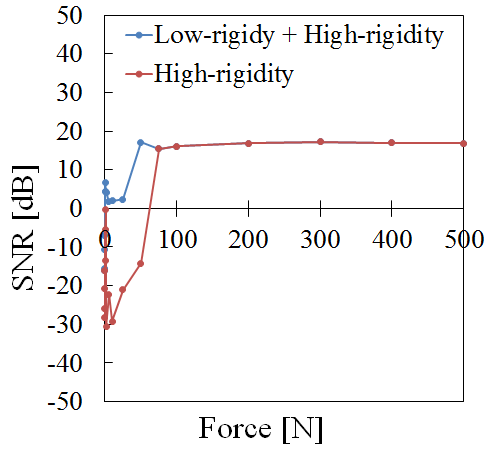
\includegraphics[scale=0.325]{pic/SN.png}}
  \subfloat[横軸:対数表示]{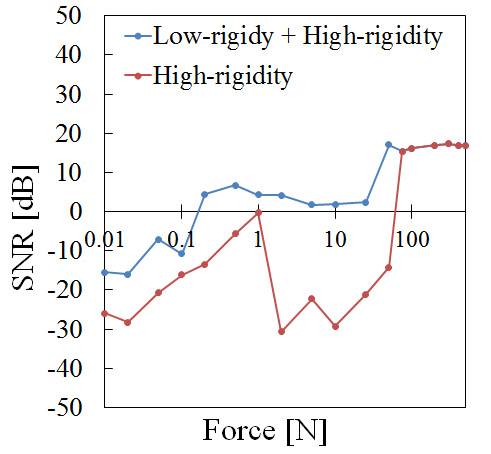
\includegraphics[scale=0.325]{pic/SNT.png}}\\
  \caption[]{SN比($F_z)$成分}\label{fig:sn}
\end{figure}
\begin{figure}%[tb]
  \centering
  \subfloat[低剛性起歪体]{\includegraphics[scale=0.325]{pic/1.png}}
  \subfloat[高剛性起歪体]{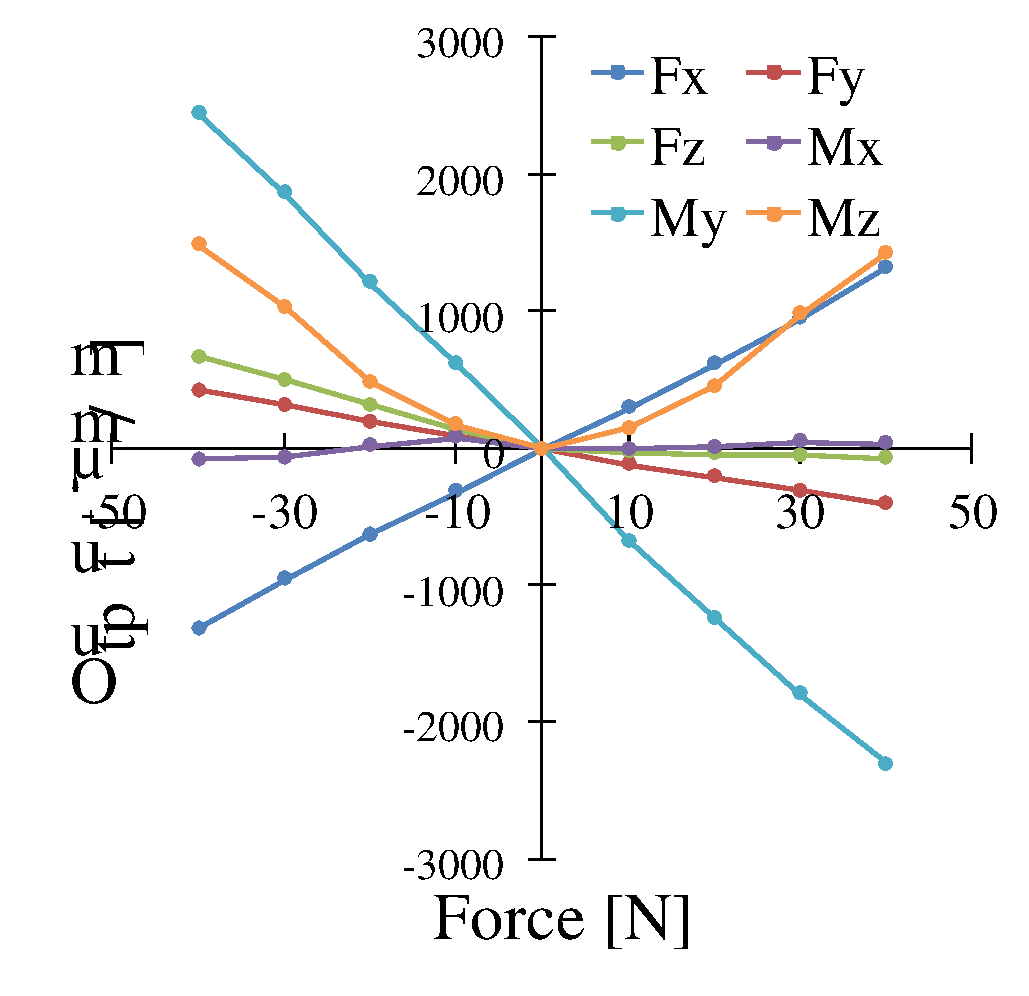
\includegraphics[scale=0.325]{pic/2.png}}\\
  \caption[]{$-F_z$を印加時のひずみ出力}\label{fig:stop}
\end{figure}
%\begin{figure}[tb]
 % \centering
 %\subfloat[$F_x$]{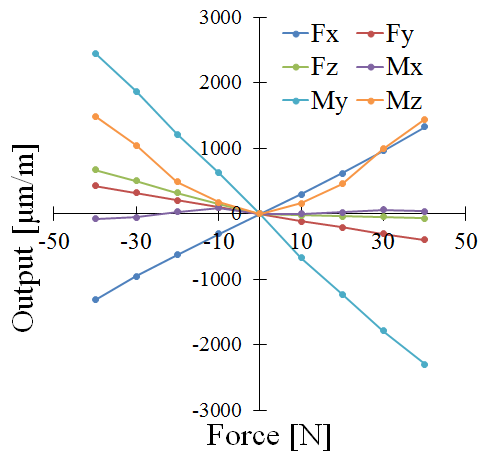
\includegraphics[scale=0.33]{pic/Sx_L.png}}
  %\subfloat[$F_y$]{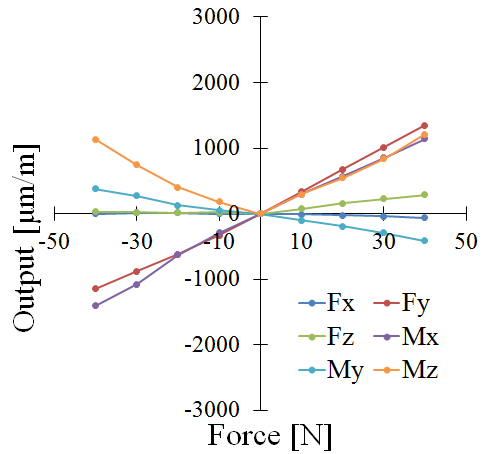
\includegraphics[scale=0.33]{pic/Sy_L.png}}\\
  %\subfloat[$F_z$]{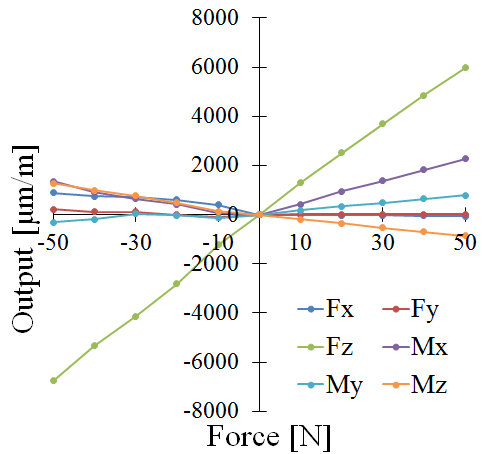
\includegraphics[scale=0.33]{pic/Sz_L.png}}
  %\subfloat[$M_x$]{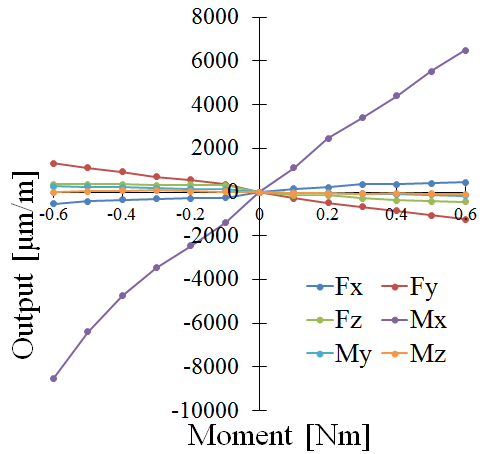
\includegraphics[scale=0.33]{pic/SMx_L.png}}\\
  %\subfloat[$M_y$]{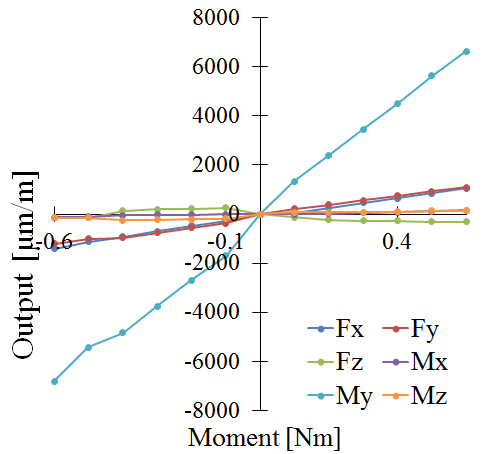
\includegraphics[scale=0.33]{pic/SMy_L.png}}
  %\subfloat[$M_z$]{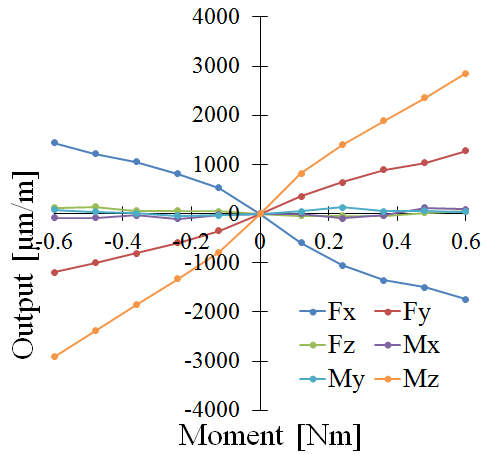
\includegraphics[scale=0.33]{pic/SMz_L.png}}\\
  %\caption[]{非線形性と他軸干渉(低剛性起歪体)}\label{fig:HTLow}
%\end{figure}
%\begin{figure}[tb]
 % \centering
 % \subfloat[$F_x$]{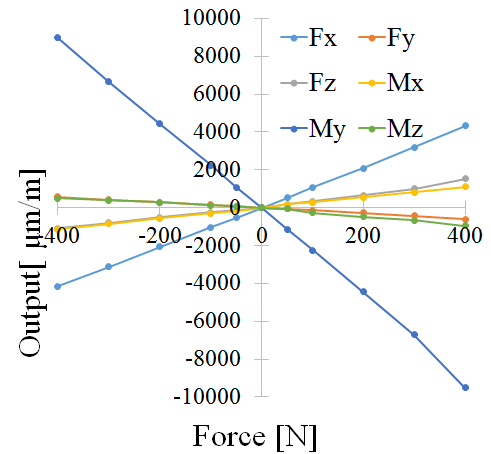
\includegraphics[scale=0.33]{pic/Sx_H.png}}
  %\subfloat[$F_y$]{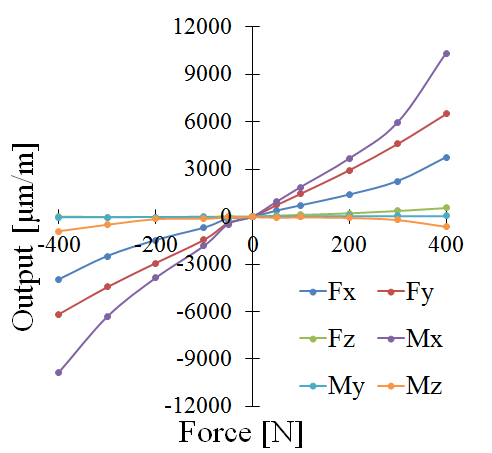
\includegraphics[scale=0.33]{pic/Sy_H.png}}\\
  %\subfloat[$F_z$]{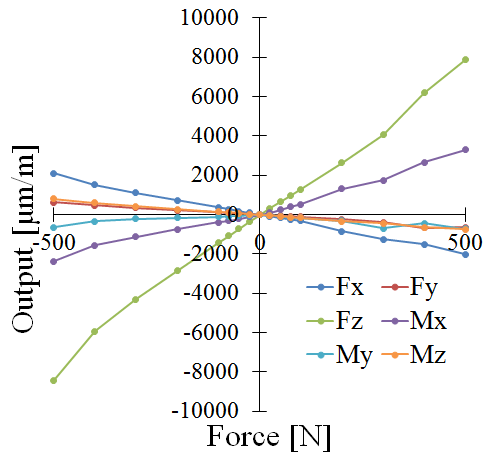
\includegraphics[scale=0.33]{pic/Sz_H.png}}
  %\subfloat[$M_x$]{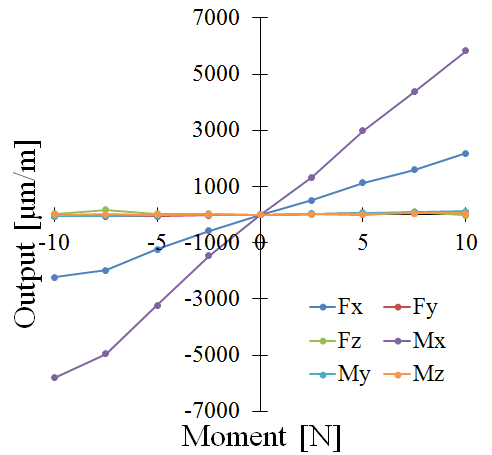
\includegraphics[scale=0.33]{pic/SMx_H.png}}\\
  %\subfloat[$M_y$]{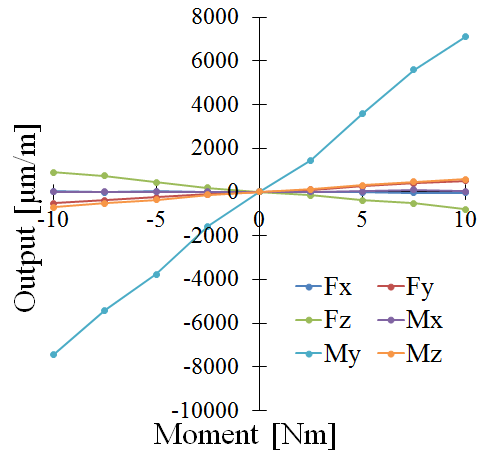
\includegraphics[scale=0.33]{pic/SMy_H.png}}
  %\subfloat[$M_z$]{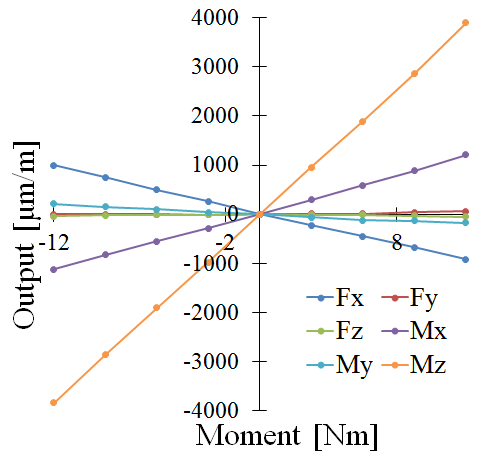
\includegraphics[scale=0.33]{pic/SMz_H.png}}\\
  %\caption[]{非線形性と他軸干渉(高剛性起歪体)}\label{fig:HTHigh}
%\end{figure}

\end{document}